\section{The phonon-assisted rate}\label{sec:13.3}

A dark-matter particle of \SI{0.35}{MeV} that transfers \SI{1.0}{keV} of momentum to silicon can deposit up to \SI{1.22}{eV}, while at that momentum transfer the cheapest zero-phonon pair along the valley axis costs about \SI{1.77}{eV} (\cref{eq:3.3-Emin}, with the bands of \cref{fig:3-si-bands}). Every event it causes therefore leaves a phonon behind, a transverse acoustic phonon of \SI{14}{meV} that carries the remaining \SI{0.94}{keV} of the valley momentum. The square of the amplitude of \cref{sec:13.2}, summed over final states, enters the rate exactly as the zero-phonon structure factor of \cref{sec:10.1} does.

\subsection{The phonon-assisted structure factor}

The structure factor counts the transitions that the density operator drives from the thermal state, \cref{eq:2.5-golden} with the transition sum \cref{eq:2.5-transum}. The off-shell window is the region $\omega \le E_{\mathrm{min}}(\vect{q}) - \delta_{\mathrm{w}}$, with $\delta_{\mathrm{w}}$ the margin of \cref{sec:8.6}, which is \SI{0.3}{eV} in silicon (\cref{sec:13.6}). Inside the off-shell window no zero-phonon pair exists at the energy deposited, and every final state contains a phonon, up to a virtual admixture of relative weight $\theta_{\mathrm{ep}}$ (\cref{sec:8.6}). The final states are those of \cref{eq:13.2-final}, and the matrix element of the density into each of them is \cref{eq:13.2-M}.

To sum over the final states, we label them by $\vect{k}$ and $\vect{Q}$, each running over the $N$ points of the zone, by the bands $c$ and $v$, the branch $\nu$, the sign, and the spin. Neither vertex flips the spin, so the spin gives a factor 2. The initial phonon state is thermal, and the average of the squared phonon matrix element is $n_{\vect{Q}\nu} + 1$ for emission and $n_{\vect{Q}\nu}$ for absorption, with $n_{\vect{Q}\nu} = n_{\mathrm{B}}(\omega_{\vect{Q}\nu})$. The electrons start in the ground state: the Fermi factor $f_v(1 - f_c)$ of each transition differs from one by terms of order $\ee^{-\Eg/2T}$. The energy delta function sets $\omega = \varepsilon_{c,\vect{k}+\vect{q}+\vect{Q}} - \varepsilon_{v\vect{k}} \pm \omega_{\vect{Q}\nu}$. The factors combine as $(2\pi/\Vol)\times2\times N^{-1}\sum_{\vect{k}\vect{Q}} = (4\pi N/\Vol)\langle\!\langle\cdots\rangle\!\rangle$ with the double zone average of \cref{eq:A.3-BZ}, and $\Vol = N\Omega$ (\cref{app:D.35} gives the thermal averages):
\begin{keyresult}[Phonon-assisted structure factor]
\begin{equation}
  S^{\mathrm{PA}}(\vect{q},\omega) = \frac{4\pi}{\Omega}\,\Bigl\langle\!\Bigl\langle\sum_\nu\sum_{cv}\sum_\pm\bigl(n_{\vect{Q}\nu} + \tfrac12 \pm \tfrac12\bigr)\,\bigl|M^\pm_{cv\nu}(\vect{k},\vect{q},\vect{Q})\bigr|^2\,\delta\bigl(\varepsilon_{c,\vect{k}+\vect{q}+\vect{Q}} - \varepsilon_{v\vect{k}} \pm \omega_{\vect{Q}\nu} - \omega\bigr)\Bigr\rangle\!\Bigr\rangle ,
  \label{eq:13.3-SPA}
\end{equation}
for $T \ll \Eg$ and $\omega$ inside the off-shell window. The phonon-assisted rate is \cref{eq:8.2-spectrum} with $\mathfrak{D}_{ee} = \pi\sigmae\FDM(q)^2/\mu_{\chi e}^2$ (\cref{eq:1.4-Vsq}) and $S = S^{\mathrm{PA}}$.
\end{keyresult}
\noindent The number of cells drops out, as it must. The double sum over $\vect{k}$ and $\vect{Q}$ contributes $N^2$, the vertex $N^{-1}$, and the volume $\Vol = N\Omega$ the last power, so that $S^{\mathrm{PA}}$ is intensive like the structure factor of a single pair.

The two signs are the two thresholds of \cref{sec:6.5}. Emission costs the phonon energy and comes with $n_{\vect{Q}\nu} + 1$; absorption gains it and comes with $n_{\vect{Q}\nu}$, and opens at energies below the gap. The weights of absorption and emission stand in the ratio $\ee^{-\omega_{\vect{Q}\nu}/T}$ of \cref{eq:6.5-ratio}. At detector temperatures the transverse acoustic phonon of \SI{15}{meV} is unoccupied ($n_{\mathrm{B}} < 10^{-74}$ below \SI{1}{K}, \cref{sec:13.1}). Only emission survives, the lower sign drops out, and \cref{eq:13.3-SPA} vanishes below the onset $E_{\mathrm{min}}^{\mathrm{PA}}(\vect{q})$ of \cref{eq:13.1-EPA}.

\Cref{eq:13.3-SPA} holds where every denominator of $M^\pm$ is bounded away from zero, and the window condition guarantees that bound: a denominator vanishes only where a first-order transition at the same $(\vect{q},\omega)$ is on shell (\cref{sec:13.2}). In the expansion of \cref{sec:8.5} the rate is quadratic in the electron--phonon vertex, $n_g = 2$, and the next order costs one power of the off-shell parameter $\theta_{\mathrm{ep}}$, 0.010 to 0.016 in silicon at the absorption edge (\cref{eq:8.5-theta}). The amplitude is unscreened, so the many-body approximation is $\mathcal{X} = \mathrm{IP}$; \cref{sec:13.4} screens both the density vertex and the pair. Beyond the window the intermediate states can be real, and the resonant paths need the widths and the finite part of \cref{sec:13.6}.

\subsection{The phonon-assisted loss function}

The fluctuation--dissipation relation \cref{eq:4.4-SL} defines a loss function for any piece of the structure factor. For the phonon-assisted piece we write
\begin{keyresult}[Phonon-assisted loss function]
\begin{equation}
  \begin{aligned}
  L^{\mathrm{PA}}(\vect{q},\omega) &= \frac{e^2}{2q^2}\bigl(1 - \ee^{-\beta\omega}\bigr)\,S^{\mathrm{PA}}(\vect{q},\omega)\\
  &= \frac{8\pi^2\alpha}{\Omega\,q^2}\,\Bigl\langle\!\Bigl\langle\sum_{\nu cv\pm}w_\pm\,\bigl|M^\pm_{cv\nu}\bigr|^2\,\delta\bigl(\varepsilon_{c,\vect{k}+\vect{q}+\vect{Q}} - \varepsilon_{v\vect{k}} \pm \omega_{\vect{Q}\nu} - \omega\bigr)\Bigr\rangle\!\Bigr\rangle ,
  \end{aligned}
  \label{eq:13.3-LPA}
\end{equation}
with $w_\pm = (1 - \ee^{-\beta\omega})(n_{\vect{Q}\nu} + \frac12 \pm \frac12)$. The rate is \cref{eq:10.2-rate} with $\bar L$ replaced by $\bar L^{\mathrm{PA}}$, its average over the directions of $\vect{q}$.
\end{keyresult}
\noindent The second form uses $e^2 = 4\pi\alpha$. The factor $1 - \ee^{-\beta\omega}$ appears once, in $L^{\mathrm{PA}}$, and \cref{eq:10.2-rate} divides it out again, so the rate carries only the phonon factors $n_{\vect{Q}\nu} + \frac12 \pm \frac12$ of \cref{eq:13.3-SPA}. Each weight $w_\pm$ is the rate of a transition minus that of its inverse, as for any dissipative response (\cref{app:D.35}). At a detector's temperature, with $\beta\omega \sim 10^4$ or more, the factor $1 - \ee^{-\beta\omega}$ and the emission factor $n_{\vect{Q}\nu} + 1$ are both one, and $L^{\mathrm{PA}}$ is $(e^2/2q^2)S^{\mathrm{PA}}$ with the emission term alone.

Since the amplitude is unscreened, $L^{\mathrm{PA}}$ is a phonon-assisted imaginary dielectric function at finite momentum, $\varepsilon_2^{\mathrm{PA}}(\vect{q},\omega)$, in the same way that the independent-particle structure factor of \cref{sec:10.1} is $(2q^2/e^2)\,\varepsilon_2^{\mathrm{IP}}$ (\cref{sec:10.2}). As $\vect{q} \to 0$ the density vertex reduces to the velocity vertex on shell (\cref{eq:3.2-optical}), and $\varepsilon_2^{\mathrm{PA}}(\vect{q},\omega)$ tends to the phonon-assisted absorption $\varepsilon_2^{\mathrm{PA}}(\omega)$ of \cref{eq:6.5-eps2PA}; \cref{sec:13.5} proves this limit and uses the measured absorption edge as the test of a computed $L^{\mathrm{PA}}$. And with the other electrons polarizing the medium, a loss function is the imaginary part of $-1/\varepsilon$, not $\varepsilon_2$; \cref{sec:13.4} shows that the phonon-assisted part then becomes $\varepsilon_2^{\mathrm{PA}}/(\varepsilon_1^0)^2$ plus the screening of the pair.

The prescriptions of \cref{sec:8.6} for adding rates apply to $L^{\mathrm{PA}}$ directly. A measured loss function or optical conductivity contains both electronic sectors, the zero-phonon line and the phonon sideband, and a computed $L^{\mathrm{PA}}$ is never added to the measured one. Below the direct gap the measured optical absorption of silicon is the phonon-assisted loss function at $\vect{q} \to 0$ and nothing else, at the temperature of the measurement. For that reason \cref{sec:13.5} has to transfer the measured absorption to millikelvin before using it in place of $L^{\mathrm{PA}}$.

A first-principles $L^{\mathrm{PA}}$ needs the bands, the density vertices and the electron--phonon vertices at three crystal momenta, $\vect{k}$, $\vect{k}+\vect{q}$ and $\vect{k}+\vect{Q}$, on fine and independent grids of $\vect{k}$ and $\vect{Q}$, as for \cref{eq:6.5-eps2PA}.

\subsection{The zero-phonon limit}

Applied at first order, the same sums over final states give back the structure factor of \cref{sec:10.1}. Without a phonon the matrix element of the density between the ground state and a pair is $\rho_{cv}(\vect{k},\vect{q})$, the final states are labeled by $\vect{k}$ alone, and the sum is $(2\pi/\Vol)\times2\times\sum_{\vect{k}}$. With $N^{-1}\sum_{\vect{k}} = \Omega\int_{\mathrm{BZ}}\dd^3k/(2\pi)^3$ the sum becomes $4\pi\int_{\mathrm{BZ}}\dd^3k/(2\pi)^3\,|\rho_{cv}|^2\,\delta(\omega - \varepsilon_{c,\vect{k}+\vect{q}} + \varepsilon_{v\vect{k}})$, which is \cref{eq:10.1-S0} term by term. The phonon-assisted structure factor has a second zone average, over the phonon wavevector, and the factor $N^{-1}$ of the electron--phonon vertex compensates that average, so the zero-phonon and phonon-assisted structure factors enter the same rate formula with the same prefactor. In the normalization of the crystal form factor, a phonon-assisted table is $q^3\Omega\bar S^{\mathrm{PA}}/(4\pi\alpha m_e^2)$, as in \cref{eq:10.1-fcrys}, and it enters the rate \cref{eq:10.1-rateiso} by addition to $|f_{\mathrm{crys}}|^2$.

The zero-phonon structure factor is the $n_g = 0$ term of the expansion in the electron--phonon vertex, and $S^{\mathrm{PA}}$ is its $n_g = 2$ term. As $g \to 0$, $M^\pm$ vanishes linearly, $S^{\mathrm{PA}}$ quadratically, the phonon-dressed sector empties, and the rate is the crystal form-factor rate of \cref{sec:10.1}. Inside the window $S^0$ is zero, since no pair exists below $E_{\mathrm{min}}(\vect{q})$, and $S^{\mathrm{PA}}$ is the whole electronic response at this order. Above $E_{\mathrm{min}}(\vect{q})$ both structure factors are present, and at order $g^2$ the two rates add with no interference term (\cref{sec:13.2}).

Adding the two rates can still double-count, because the two sectors share one sum rule. The electron--phonon Hamiltonian is a function of the electron positions and commutes with the density, so the $f$-sum of the electron density, \cref{eq:4.3-firstmoment}, holds at every order in $g$; the two electronic sectors together carry it up to a part in $10^3$ (\cref{sec:8.6}). The first moment of $S^{\mathrm{PA}}$ is positive, and the zero-phonon sector loses the same amount at the same order, through the self-energies and vertex corrections of its pairs. If the zero-phonon rate is computed with the bare bands and $|\rho_{cv}|^2$ and $S^{\mathrm{PA}}$ is added to it, the sum overshoots the $f$-sum by the first moment of $S^{\mathrm{PA}}$, a relative excess of order $\theta_{\mathrm{ep}}$. The renormalized zero-phonon response of \cref{sec:13.7} removes this overshoot. Inside the window there is no overshoot, because the zero-phonon line has no weight to lose there.

\subsection{The onset exponent}

Near its threshold the phonon-assisted rate is a power of the energy above it, and the power is fixed by counting the free momenta of the final state. Take a fixed $\vect{q}$, $T \to 0$, and an energy deposited just above the onset of \cref{eq:13.1-EPA}, at a distance $x = \omega - E_{\mathrm{min}}^{\mathrm{PA}}(\vect{q})$ above the onset. The hole lies near the valence-band maximum and the electron near the bottom of the valley $\vect{k}_{\mathrm{c}}$, at small momenta $\vect{\kappa}_{\mathrm{h}}$ and $\vect{\kappa}_{\mathrm{e}}$ from the extrema, and the phonon wavevector is $\vect{Q}^* + \vect{\kappa}_{\mathrm{e}} - \vect{\kappa}_{\mathrm{h}}$ with $\vect{Q}^* = \vect{k}_{\mathrm{c}} - \vect{q}$. The final-state energy above the onset is
\begin{equation*}
  \frac{\kappa_{\mathrm{e}}^2}{2m^*_{\mathrm{d}}} + \frac{\kappa_{\mathrm{h}}^2}{2m_{\mathrm{h}}} + \vect{u}_\nu\cdot(\vect{\kappa}_{\mathrm{e}} - \vect{\kappa}_{\mathrm{h}}) + O(\kappa^2\,\partial^2\omega_\nu) ,
\end{equation*}
with $\vect{u}_\nu$ the group velocity of the phonon at $\vect{Q}^*$ and the valley written with its density-of-states mass, as in \cref{sec:6.5}. The linear term tilts the minimum: completing the square lowers the minimum by $\frac12M_{\mathrm{eh}}u_\nu^2$, with $M_{\mathrm{eh}} = 1.19\,m_e$ the pair mass of \cref{sec:13.1}. This lowering is the one that \cref{sec:13.1} found to be below \SI{0.02}{meV} at the onset mass; at $|\vect{q}| = \SI{1.0}{keV}$ it is \SI{0.02}{meV} for the transverse acoustic branch and \SI{0.18}{meV} for the longitudinal one. The curvature of the phonon branch is a percent of $1/M_{\mathrm{eh}}$ and changes the pocket masses by about a percent. The final states then form two independent parabolic pockets, because the phonon takes up any momentum mismatch. Their joint density of states is \cref{eq:6.5-joint}. With $M^\pm$ constant across the pockets, at its value $M_\nu$ at the extrema, \cref{eq:13.3-SPA} becomes, per valley, branch and valence band,
\begin{equation}
  S^{\mathrm{PA}}(\vect{q},\omega) \simeq \frac{\Omega\,(m^*_{\mathrm{d}}m_{\mathrm{h}})^{3/2}}{4\pi^2}\,|M_\nu|^2\,x^2\,\Theta(x) .
  \label{eq:13.3-near}
\end{equation}
At fixed $\vect{q}$ the rate rises as the square of the energy above its onset, the Hall--Bardeen--Blatt law \cref{eq:6.5-edge} at finite momentum transfer.

The rate of a detector that does not resolve the direction of $\vect{q}$ uses $\bar S^{\mathrm{PA}}$, and the average over directions adds powers of $x$. The onset depends on the direction through $\vect{Q}^*$. Let $\theta_q$ be the angle between $\vect{q}$ and the valley axis, take $q < k_{\mathrm{c}}$ and expand for small $\theta_q$. The phonon wavevector lengthens, $|\vect{Q}^*|^2 = (k_{\mathrm{c}} - q)^2 + 2k_{\mathrm{c}}q(1 - \cos\theta_q) \simeq (k_{\mathrm{c}} - q)^2 + k_{\mathrm{c}}q\,\theta_q^2$, and it tilts away from the axis by $\theta_Q \simeq q\theta_q/(k_{\mathrm{c}} - q)$. With the phonon energy near the axis written as a function of $|\vect{Q}|$ and $\theta_Q$, the onset is
\begin{equation}
  E_{\mathrm{min}}^{\mathrm{PA}}(\theta_q) \simeq \Eg + \omega_\nu(k_{\mathrm{c}} - q) + \varkappa_\nu\theta_q^2 , \qquad
  \varkappa_\nu = \frac{\omega_\nu'\,k_{\mathrm{c}}q}{2(k_{\mathrm{c}} - q)} + \frac{\partial^2_{\theta_Q}\omega_\nu}{2}\,\frac{q^2}{(k_{\mathrm{c}} - q)^2} ,
  \label{eq:13.3-Eth}
\end{equation}
where $\omega_\nu'$ is the slope of the branch along the axis and $\partial^2_{\theta_Q}\omega_\nu$ its curvature in the tilt angle at fixed $|\vect{Q}|$, both at $|\vect{Q}| = k_{\mathrm{c}} - q$. The first term comes from the longer phonon wavevector and is positive for a branch that rises away from $\mathrm{\Gamma}$; the second is the anisotropy of the branch. Where $\varkappa_\nu > 0$ the valley axis is an isolated minimum of the onset, and only a cone of half-angle $(x/\varkappa_\nu)^{1/2}$ around it contributes at energy $x$ above the onset. Integrating \cref{eq:13.3-near} over that cone, as \cref{we:13-onset-exp} does, gives one more power of $x$.

The two powers, $x^2$ at fixed $\vect{q}$ and one more after the average, are instances of one rule. If the final-state energy has an isolated quadratic minimum in $D$ free variables, the volume below $x$ grows as $x^{D/2}$ and the density of states as $x^{D/2 - 1}$. If $|M|^2$ vanishes at the minimum as the square of the distance from it, one more power enters. Two free pockets give $D = 6$ and $x^2$, and the two angles of $\hat{\vect{q}}$ make $D = 8$ and $x^3$. A bound exciton with a phonon has only its center-of-mass momentum free, $D = 3$, and its replica rises as $x^{1/2}$ at fixed $\vect{q}$ and as $x^{3/2}$ after the average (\cref{sec:13.8}). The power of $x$ in $\bar S^{\mathrm{PA}}$, and so in $\bar L^{\mathrm{PA}}$ and in the spectrum at fixed $|\vect{q}|$, is the \emph{onset exponent} $p_{\mathrm{on}}$.

Symmetry decides whether $M_\nu$ vanishes at the minimum. In silicon, with $\vect{q}$ on a valley axis, the vectors $\vect{q}$, $\vect{Q}^*$ and $\vect{k}_{\mathrm{c}}$ all lie on the [100] line, and the operations that leave this line fixed form the group $C_{4v}$. The electron at the bottom of the valley belongs to the identity representation $\Delta_1$ of $C_{4v}$, and the threefold valence maximum $\Gamma_{25}'$ splits on the line into $\Delta_2' \oplus \Delta_5$~\cite[Chap.~2]{yu2010fundamentals}. The density vertex with no reciprocal-lattice vector added to $\vect{q}$ is invariant ($\Delta_1$): an operation with a fractional translation $\vect{\tau}$ multiplies it by $\ee^{-\ii\vect{q}\cdot\vect{\tau}}$, and this phase cancels against those of the two Bloch states, as \cref{we:13-glide} shows for the mirror. A longitudinal acoustic displacement lies along the axis and is in phase on the two atoms of the cell. Every operation that fixes the axis maps the axis onto itself and the two atoms onto each other or themselves, so it leaves the longitudinal acoustic displacement unchanged, and that displacement is $\Delta_1$ as well; the longitudinal optical displacement is $\Delta_2'$, and the transverse pairs are $\Delta_5$. An amplitude is a number and is nonzero only if the product of the representations of electron, vertex, phonon and hole contains $\Delta_1$ (\cref{eq:C.17-orth}). For the longitudinal acoustic phonon the product is $\Delta_1\otimes\Delta_1\otimes\Delta_1\otimes(\Delta_2' \oplus \Delta_5) = \Delta_2' \oplus \Delta_5$, which does not contain $\Delta_1$. The transverse branches and the longitudinal optical one are allowed, because $\Delta_5\otimes\Delta_5$ and $\Delta_2'\otimes\Delta_2'$ contain $\Delta_1$.

The forbidden branch rises one power later. Off the axis its amplitude grows linearly with the distance from the axis, $|M|^2$ grows quadratically, and the longitudinal acoustic onset is a kink with $p_{\mathrm{on}} = 4$ on top of the transverse acoustic edge with $p_{\mathrm{on}} = 3$. Spin--orbit coupling mixes the valence representations, lifts the zero of the longitudinal acoustic amplitude, and leaves a part with $p_{\mathrm{on}} = 3$. We estimate the relative weight of this part as below $10^{-4}$, from the spin--orbit lift of the zero-phonon vertex on the same axis, $|\rho_{cv}|^2 = 3.6\times10^{-6}$ against an allowed 0.150 (\cref{sec:13.9-glide}). Beyond $|\vect{q}| = 2\pi/a = \SI{2.28}{keV}$, halfway between the valley at $0.85\,\mathrm{X}$ and the image of the opposite valley at $1.15\,\mathrm{X}$, the nearest pocket is that image, reached with the reciprocal-lattice vector $(2\pi/a)(2,0,0)$ inside the vertex. There the vertex picks up the glide phase of \cref{eq:C.17-parity} and transforms as $\Delta_2'$, the longitudinal optical branch becomes the forbidden one, and the longitudinal acoustic branch is allowed. Its minimum, however, lies off the axis, where the vertex does not vanish, so every branch of that class has $p_{\mathrm{on}} = 3$.

Whether the minimum of each branch lies on the axis depends on the sign of $\varkappa_\nu$. With the silicon dispersion of \cref{sec:5.2}, the transverse acoustic onset has its minimum on the axis for $|\vect{q}| < \SI{1.34}{keV}$; above \SI{1.34}{keV}, the anisotropy term of \cref{eq:13.3-Eth} dominates and the minima move off the axis into the $\{001\}$ planes. The longitudinal acoustic branch rises steeply and keeps its minimum on the axis. The optical branches fall away from $\mathrm{\Gamma}$, the first term of $\varkappa_\nu$ is negative, and their minima lie far off the axis: at $|\vect{q}| = \SI{1.0}{keV}$ the lowest optical onset over all directions is \SI{44}{meV} above $\Eg$, against \SI{60}{meV} on the axis. None of these displacements of the minima changes an exponent. Off the axis, cubic symmetry leaves isolated minima at which the vertex is generically nonzero, and $p_{\mathrm{on}} = 3$; a minimum spread over a ring around the axis would give $5/2$, but the anisotropy of a cubic crystal breaks the ring. In germanium the valleys lie at L on the threefold axes, the group of the line is $C_{3v}$, the valence maximum splits into $\Lambda_1 \oplus \Lambda_3$, the electron is $\Lambda_1$ and the phonons are $\Lambda_1$ (longitudinal) and $\Lambda_3$ (transverse). Every branch is allowed, and $p_{\mathrm{on}} = 3$ throughout. The two transverse acoustic branches of germanium are degenerate on the [111] axis and split linearly away from it, so their minimum is never on the axis.

\begin{keyresult}[Onset exponent]
Inside the off-shell window, at zero temperature and fixed $|\vect{q}|$, the direction-averaged phonon-assisted loss function rises above its onset as $x^{p_{\mathrm{on}}}$ with
\begin{equation}
  \begin{aligned}
  p_{\mathrm{on}} &= 3 \quad \text{(Si: transverse acoustic edge, optical branches; Ge: all branches)}, \\
  p_{\mathrm{on}} &= 4 \quad \text{(Si: longitudinal acoustic kink)},
  \end{aligned}
  \label{eq:13.3-pon}
\end{equation}
two at a fixed direction of $\vect{q}$, and $3/2$ for an exciton replica.
\end{keyresult}

\Cref{fig:13-paloss} shows the exponents in a model of silicon at $|\vect{q}| = \SI{1.0}{keV}$, with the onsets taken from the computed dispersion over the whole sphere of directions. Panel (b) gives the range of the exponents. The averaged transverse acoustic component follows $x^3$ within \SI{10}{\percent} for $x < \SI{1.3}{meV}$, and its local exponent has drifted only to 3.3 at \SI{10}{meV}; the longitudinal acoustic one follows $x^4$ for $x < \SI{2.4}{meV}$. The average over directions also reduces the strength of the transverse acoustic component, by a factor $1.2\times10^{-3}$ at \SI{0.1}{meV} above the onset (\cref{we:13-onset-exp}).

\begin{figure}[tbp]
  \centering
  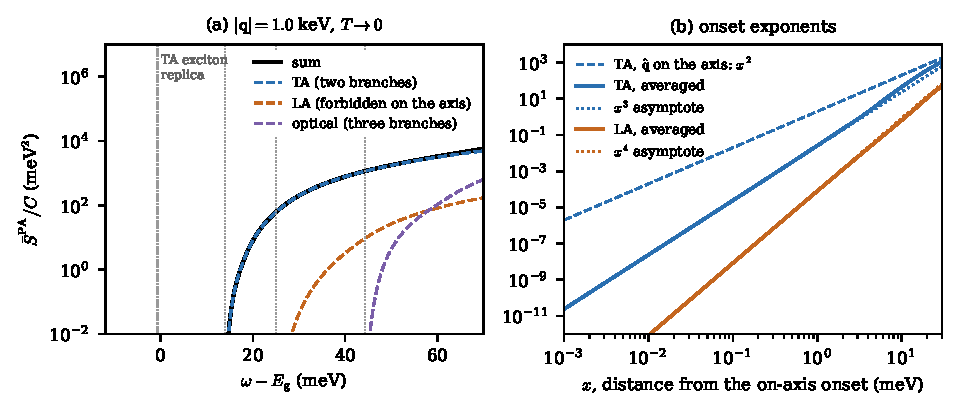
\includegraphics[width=\linewidth]{figures/ch13/fig13_3.pdf}
  \caption{The phonon-assisted structure factor of silicon near its threshold, averaged over the directions of $\vect{q}$ at $|\vect{q}| = \SI{1.0}{keV}$, at zero temperature (emission only), in units of a common coefficient $C$. Model: one valley at $\vect{k}_{\mathrm{c}} = 0.85\,(2\pi/a)$, parabolic pockets and the fixed-$\vect{q}$ form \cref{eq:13.3-near}, with the onset $\Eg + \omega_\nu(\vect{k}_{\mathrm{c}} - \vect{q})$ computed in every direction from the PBE force constants of \cref{sec:5.2}, whose transverse acoustic energy at X is \SI{17.06}{meV} against \SI{18.57}{meV} measured. Every branch is given the same $|M_\nu|^2 = C$, except the longitudinal acoustic one, which is given $C\sin^2\theta_Q$ because its amplitude vanishes on the valley axis; the relative heights are therefore illustrative. The tilt of the pair minimum (at most \SI{0.18}{meV}) is neglected. (a) Components against $\omega - \Eg$: the transverse acoustic edge at \SI{13.98}{meV}, the longitudinal acoustic kink at \SI{25.00}{meV}, and the optical onset at \SI{44.1}{meV}, whose minimum lies far off the axis (dotted lines). The dash-dotted line marks the exciton replica of the transverse acoustic edge, $E_x^b = \SI{14.7}{meV}$ lower, whose strength is not modeled. (b) Each acoustic component against the distance $x$ from its own onset. With $\vect{q}$ held on the axis the transverse acoustic component grows as $x^2$ (dashed). Averaged over directions it grows as $x^3$ (solid), and the longitudinal acoustic one as $x^4$; dotted lines are the asymptotes of \cref{we:13-onset-exp}. The window condition holds over the whole plot: at this $|\vect{q}|$ the zero-phonon pair continuum starts \SI{0.60}{eV} above $\Eg$ (PBE bands of \cref{sec:3.3} with the measured gap).}
  \label{fig:13-paloss}
\end{figure}

The exponents also require the onset itself to lie inside the window. At the onset the pair sits at the band extrema and the phonon takes all of $\vect{Q}^*$, while the zero-phonon edge at the same $\vect{q}$ lies $|\vect{Q}^*|^2/2M_{\mathrm{eh}}$ above $\Eg$ (\cref{eq:3.3-Eminpar}). The window condition $\Eg + \omega_\nu(\vect{Q}^*) \le E_{\mathrm{min}}(\vect{q}) - \delta_{\mathrm{w}}$ then reads $|\vect{Q}^*|^2 - 2M_{\mathrm{eh}}c\,|\vect{Q}^*| - 2M_{\mathrm{eh}}\delta_{\mathrm{w}} \ge 0$ for a branch $\omega_\nu = c|\vect{Q}|$, that is,
\begin{equation*}
  |\vect{Q}^*| \ge M_{\mathrm{eh}}c + \bigl(M_{\mathrm{eh}}^2c^2 + 2M_{\mathrm{eh}}\delta_{\mathrm{w}}\bigr)^{1/2} .
\end{equation*}
With a margin $\delta_{\mathrm{w}} = \SI{0.3}{eV}$, five times the top of the phonon band (\cref{sec:13.6} fixes the margin), and the phase velocity of the transverse acoustic branch at the bound, \SI{5.0}{km.s^{-1}}, the bound is \SI{0.31}{\angstrom^{-1}}, or \SI{0.615}{keV}. In silicon the exponents of \cref{eq:13.3-pon} therefore hold for $|\vect{q}| \le k_{\mathrm{c}} - \SI{0.615}{keV} = \SI{1.33}{keV}$ for parabolic valleys, and for $|\vect{q}| \le \SI{1.27}{keV}$ with the computed bands (\cref{sec:13.6}); over this whole range the transverse acoustic minimum lies on the axis. Closer to the valley the onset falls into the edge band of \cref{sec:13.6}, at the edge of the window, where the phonon-assisted rate is not separately defined and therefore has no exponent of its own.

\begin{workedexample}{The onset exponent from the joint density of states}\label{we:13-onset-exp}
Take silicon at $|\vect{q}| = \SI{1.0}{keV}$, near the valley axis [100], with $k_{\mathrm{c}} = 0.85\,(2\pi/a) = \SI{1.94}{keV}$. On the axis the phonon carries $k_{\mathrm{c}} - q = \SI{0.94}{keV}$, or \SI{0.48}{\angstrom^{-1}} $= 0.41\,\mathrm{X}$, where the computed dispersion of \cref{sec:5.2} gives $\omega_{\mathrm{TA}}(\vect{Q}^*) = \SI{13.98}{meV}$ and $\omega_{\mathrm{LA}}(\vect{Q}^*) = \SI{25.00}{meV}$. The onset $\Eg + \omega_{\mathrm{TA}}(\vect{Q}^*) = \SI{1.184}{eV}$ is reached by dark matter heavier than \SI{0.341}{MeV}, since $qv_{\mathrm{max}} - q^2/2\mchi$ must exceed it with $qv_{\mathrm{max}} = \SI{2.650}{eV}$. The zero-phonon edge at this $\vect{q}$ lies \SI{0.60}{eV} above $\Eg$ on the computed bands of \cref{fig:3-si-bands} (the parabola \cref{eq:3.3-Eminpar} gives \SI{0.73}{eV}), so the window extends to \SI{0.30}{eV} above $\Eg$, well beyond the energies considered here.

\emph{Fixed direction.} With $\vect{q}$ on the axis, \cref{eq:13.3-near} gives $S^{\mathrm{PA}} = Cx^2$ for each transverse acoustic branch, $C = \Omega(m^*_{\mathrm{d}}m_{\mathrm{h}})^{3/2}|M_{\mathrm{TA}}|^2/4\pi^2$, with $m^*_{\mathrm{d}} = 0.322\,m_e$. This is the $x^2$ of \cref{eq:6.5-joint}: the two pockets give six free momenta.

\emph{The curvature of the onset.} The transverse acoustic slope at \SI{0.48}{\angstrom^{-1}} is $\omega_{\mathrm{TA}}' = \SI{16.9}{meV.\angstrom}$, and the first term of \cref{eq:13.3-Eth} is
\begin{equation*}
  \frac{\omega_{\mathrm{TA}}'\,k_{\mathrm{c}}q}{2(k_{\mathrm{c}} - q)} = \SI{16.9}{meV.\angstrom}\times\frac{0.983\times\SI{0.507}{\angstrom^{-2}}}{2\times\SI{0.477}{\angstrom^{-1}}} = \SI{8.85}{meV} .
\end{equation*}
The anisotropy of the branch lowers $\varkappa$. Evaluated on a cone $\theta_q = \SI{0.02}{rad}$ around the axis, the lower transverse acoustic branch has $\varkappa$ between 2.3 and \SI{8.5}{meV} depending on the azimuth $\phi$, the upper one between 18 and \SI{24}{meV}, and the longitudinal acoustic one \SI{16.8}{meV} in every direction. All values of $\varkappa$ are positive: the axis is a minimum.

\emph{The average.} For an onset $\varkappa\theta_q^2$ above its minimum, the average over the sphere of directions, $\bar S = (4\pi)^{-1}\int\dd\phi\,\sin\theta_q\,\dd\theta_q\,S$, is dominated by small $\theta_q$, where $\sin\theta_q \simeq \theta_q$. With $u = \varkappa\theta_q^2$,
\begin{equation*}
  \frac{1}{4\pi}\int_0^{2\pi}\!\dd\phi\int\theta_q\,\dd\theta_q\,C\bigl(x - \varkappa\theta_q^2\bigr)^2\Theta = \frac{C}{4\pi}\int_0^{2\pi}\!\dd\phi\,\frac{1}{2\varkappa}\int_0^x\dd u\,(x - u)^2 = \frac{C\,x^3}{12}\Bigl\langle\frac{1}{\varkappa}\Bigr\rangle_{\!\phi} ,
\end{equation*}
with $\langle 1/\varkappa\rangle_\phi$ the average over the azimuth: \SI{0.240}{meV^{-1}} and \SI{0.047}{meV^{-1}} for the two transverse branches. The exponent has risen from 2 to 3, and $p_{\mathrm{on}} = 3$.

\emph{The forbidden branch.} For the longitudinal acoustic phonon $|M|^2 = C\sin^2\theta_Q \simeq C\,[q/(k_{\mathrm{c}} - q)]^2\theta_q^2$, and the extra $\theta_q^2 = u/\varkappa$ in the integrand gives $\int_0^x u(x - u)^2\dd u = x^4/12$, so
\begin{equation*}
  \bar S_{\mathrm{LA}} = \frac{C\,x^4}{48}\Bigl(\frac{q}{k_{\mathrm{c}} - q}\Bigr)^2\Bigl\langle\frac{1}{\varkappa^2}\Bigr\rangle_{\!\phi} ,
\end{equation*}
and $p_{\mathrm{on}} = 4$.

\emph{The cost of the average.} Per valley, the ratio of the averaged to the on-axis transverse acoustic structure factor is $(x/24)(\langle1/\varkappa\rangle_1 + \langle1/\varkappa\rangle_2)$ for the two branches, $1.2\times10^{-3}$ at $x = \SI{0.1}{meV}$. Only a cone of solid angle $\pi x/\varkappa$ around the valley axis is open, a fraction $x/4\varkappa$ of the sphere.
\end{workedexample}

At fixed $|\vect{q}|$ the halo enters the rate through $q^3\eta(\vmin)\FDM^2$ in \cref{eq:10.2-rate}, which is smooth across an onset as long as $\vmin < v_{\mathrm{max}}$. The spectrum contributed by each $|\vect{q}|$ therefore rises with the same exponent as $\bar L^{\mathrm{PA}}$. The integral over $|\vect{q}|$ smooths the spectrum further, because the onset moves with $|\vect{q}|$; \cref{sec:13.9-onset} combines these factors into the dependence of the rate on the dark-matter mass at the onset.
